\documentclass[12pt, a4paper]{extarticle}
\usepackage[left=3cm, right=2cm, top=2cm, bottom=2cm, bindingoffset=0cm]{geometry}
\usepackage{minted}
\usepackage{extsizes} 
\usepackage{kantlipsum} 
\usepackage{algorithm}
\usepackage{algpseudocode}
\usepackage{tikz}
\usepackage[T2A]{fontenc} % Поддержка русских букв
\usepackage[utf8]{inputenc}
\usepackage[english, russian]{babel}
\usepackage{amssymb}
\usepackage{amsmath}
\usepackage{amsthm}
\newcommand{\E}{\mathop{\mathbb{E}}}
\DeclareMathOperator*{\argmax}{arg\,max}
\usepackage{mathcomp}
\usepackage{amsfonts}
\usepackage{xcolor}
\usepackage{hyperref}
\usepackage{graphicx}
\usepackage{wrapfig}
\graphicspath{}
\definecolor{linkcolor}{HTML}{660066} % цвет ссылок
\definecolor{urlcolor}{HTML}{008B8B} % цвет гиперссылок
\definecolor{citecolor}{HTML}{008B8B} % цвет ссылок на литературу
\definecolor{background}{HTML}{F0F8FF} % цвет подкладки кода
\hypersetup{pdfstartview=FitH, linkcolor=linkcolor, urlcolor=urlcolor, colorlinks=true, citecolor=citecolor}
\theoremstyle{definition}
\newtheorem{definition}{Определение}[section]
\AfterEndEnvironment{definition}{\noindent\ignorespaces}


\date{June 2019}

\begin{document}

\thispagestyle{empty}
\begin{center}
	\textbf{ПРАВИТЕЛЬСТВО РОССИЙСКОЙ ФЕДЕРАЦИИ}\\
	\vspace{2ex}
	\textbf{Федеральное государственное автономное\\ образовательное учреждение высшего образования}

	\vspace{2ex}

	\textbf{Национальный исследовательский университет \\ ''Высшая школа экономики''}

	\vspace{8ex}
	\begin{flushright}
	Факультет экономических наук\\
	Образовательная программа ''Экономика''
	\end{flushright}
\end{center}
\vspace{9ex}

\begin{center}
	{\textbf{КУРСОВАЯ РАБОТА
	}}
	\vspace{1ex}

	На тему ''Применение обучения с подкреплением в экономическом моделировании''
\end{center}
	\vspace{1ex}
\begin{flushright}
	\noindent
	Студент группы БЭК-162\\Даниелян Всеволод Эдуардович\\
	\vspace{13ex}
	Научный руководитель:\\
	Старший преподаватель Демешев Борис Борисович

\end{flushright}

	\vfill

\begin{center}
		Москва 2019

\end{center}
\newpage
\tableofcontents
\clearpage

\section{Введение}
Обучение с подкреплением представляет собой разновидность машинного обучения, сконцентрованную на взаимодействии агентов, максимизирующих свои совокупные вознаграждения, с окружением. Гибкость постановки проблемы позволяет с успехом применять алгоритмы обучения с подкреплением к самому широкому спектру задач --- от игры в Старкрафт \cite{alphastarblog} до управления квадрокоптером \cite{hwangbo2017control}.

В этой работе я рассматриваю возможность применения обучения с подкреплением в экономическом моделировании на примере задачи о динамической дуополии Курно. Цель работы - продемонстрировать, как достижение экономического равновесия в динамической дуополии Курно может быть объяснено через последовательное взаимодействие друг с другом и средой независимо обучающихся агентов. 

В качестве алгоритма обучения агентов я использовал MADDPG, который является \cite{lideep} одним из наиболее продвинутых на настоящий момент алгоритмов обучения с подкреплением для окружений с несколькими агентами.



\newpage
\section{Основная часть}
\subsection{Основные концепции}
В обучении с подкреплением главными действующими лицами являются агенты и окружение. В каждый момент времени $t$ агент получает какие-то наблюдения $o_t$ о состоянии окружения $s_t$, совершает действие $a_t$, получает вознаграждение $r_t = R(s_{t},a_t,s_{t+1})$ в зависимости от состояния и действия, и переходит в следующее состояние $s_{t+1}$. Для удобства состояние и действие текущего периода могут обозначаться как просто $s$ и $a$, а будущего как $s'$ и $a'$.  

Траектория $\tau$ - это последовательность состояний и действий:
\begin{equation}
    \tau = (s_0,a_0,s_1,a_1,\ldots).
\end{equation}

Переход из состояния в состояние осуществляется в соответствии с законами, которым подчиняется окружение, и зависисит от последнего совершенного действия. Функция перехода может быть детерминистической:
\begin{equation}
    s' = f(s,a),
\end{equation}
или стохастической:
\begin{equation}
    s' \sim P(\cdot|s,a).
\end{equation}

Формализацией такого последовательного процесса принятия решений являются марковские процессы принятия решений (Markov Decision Processes --- MDP). 
\begin{definition}
MDP --- это кортеж, $\langle S, A, R, P, \rho_{0} \rangle$, где \begin{itemize}
    \item $S$ - множество состояний,
    \item $A$ - множество действий,
    \item $R: S \times A \times S \mapsto \mathbb{R}$, где $r_{t} = R(s_{t},a_t,s_{t+1})$,
    \item \label{markov} $P: S\times A \mapsto \mathcal{P}(S)$, где $P(s_{t+1}|s_{t}, a_t)$ --- функция, задающая вероятность перехода из $s_t$ в $s_{t+1}$. При этом $P$ подчиняется марковскому свойству, то есть $P(s_{t+1}|s_{t}, a_t, s_{t-1}, a_{t-1}, \ldots) = P(s_{t+1}|s_{t}, a_t)$.
\end{itemize}
\end{definition}

Почти все алгоритмы обучения с подкреплением принимают в качестве предпосылки марковское свойство. Интуиция тут такова --- мы хотим быть уверены, что вся информация, необходимая для принятия решения, содержится в состоянии $s$ текущего периода. С теоретической точки зрения, марковское свойство используется в доказательствах сходимости алгоритмов там, где оно вообще может быть получено. 

Агенты в рамках MDP совершают действия в соответсвии со своей стратегией. Если стратегия детерминистическая, то она обычно обозначается как $\mu$, и представляет собой отображение из множества состояний в множество действий:
\begin{equation} \label{mu}
    a_t = \mu(s_t)
\end{equation}
Если стратегия стохастическая, то она обычно обозначается как $\pi$ и представляет собой условное распределение над пространством действий:
\begin{equation}
a_t\sim \pi(\cdot| s_t)
\end{equation}

Далее мы часто будем иметь дело с аппроксимацией стратегий, в первую очередь с использованием нейросетей. Мы параметризуем функцию стратегии каким-то набором параметров (в случае нейросети это будут веса нейросети), обозначаемых обычно $\theta$ или $\phi$. Параметризованные таким образом стратегии соответственно обозначаются как:
\begin{equation}
    a_t = \mu_{\theta}(s_t) 
    \end{equation}
\begin{equation}
    a_t \sim \pi_{\theta}(\cdot|s_t)
    \end{equation}
    
Нам часто будет важно знать ожидаемое вознаграждение, если мы будем следовать стратегии $\pi$ начиная с текущего состояния и до конца траектории (если траектория конечна):
\begin{equation}
    V^{\pi}(s)=\E_{\tau \sim \pi} \left[R(\tau) | s_0 = s \right],
\end{equation}
или начиная с текущего состояния $s$, с учетом того, что мы совершили в нем определенное действие $a$:
\begin{equation}
    Q^{\pi}(s,a)=\E_{\tau \sim \pi} \left[R(\tau) | s_0 = s, a_0 = a \right].
\end{equation}
Здесь $R(\tau) = \sum^{\infty}_{t=0}\gamma^t r_t$ --- дисконтированная сумма вознаграждений, полученных агентом после прохождения траектории $\tau$. 

Задача обучения с подкреплением - выучить стратегию, максимизирующую математическое ожидание будущих вознаграждений:
\begin{equation}
    \pi^{*}=\argmax_{\pi}J(\pi)=\argmax_{\pi} \E_{\tau \sim \pi}\left[R(\tau)\right]
\end{equation}

\subsection{Уравнения Беллмана и Q-learning}
Q-функции текущего и будущего периода связаны следующим соотношением, известным как уравнение Беллмана:
\begin{equation} 
    Q^{\pi}(s,a) = \E\left[r(s,a) + \gamma  \E_{a' \sim \pi} \left[ Q(s',a') \right]|s, a \right]
\end{equation}

Для оптимальной стратегии уравнения Беллмана выглядят следующим образом:
\begin{equation} \label{opt_bell}
    Q^{*}(s,a) = \E \left[r(s,a) + \gamma  \max_{a'}  Q^{*}(s',a') | s, a \right].
\end{equation}

На форме уравнений Беллмана и основана идея глубокого Q-обучения (Q-learning). Мы можем аппроксимировать Q-функцию нейросетью, и обучить ее с помощью минимизации следующей функции потерь:
\begin{equation} \label{q-loss}
    L(\theta) = \E_{s,a,r,s'} \left[ (Q_{\theta}^{^*}(s,a) - y)^2  \right]
    \end{equation}
\begin{equation}
    y = r(s,a) + \gamma  \max_{a'}  Q^{*}(s',a'),
\end{equation}
где $\theta$ - параметры аппроксимирующей функции (веса нейросети).

Действительно, если мы знаем, что для оптимальной статегии должно выполняться соотношение \ref{opt_bell}, то минимизация функции потерь \ref{q-loss} должна приблизить нашу аппроксимацию к оптимальной Q-функции.
Для понимания функции потерь \ref{q-loss} может помочь и следующая интуиция: в $y$, в отличие от $Q(s,a)$ фигурирует актуальное вознаграждение $r$. Благодаря этому сам $y$ ближе к реальной Q-функции, чем $Q(s,a)$, и минимизируя функцию потерь, мы приближаем таким образом нашу аппроксимацию к тому, что мы аппроксимируем. Соответственно $y$ выступает в качестве цели, к которой мы хотим приблизиться. 

Сама минимизация как правило выполняется с помощью стохастического градиентного спуска, или подобного ему алгоритма. Следует учесть, что при взятии градиента функции потерь, $y$ обычно полагают константой, хотя $Q_{\theta}(s',a')$ зависит от параметров, по которым мы берем градиент. Такую технику называют полу-градиентом (semi-gradient) в главе 9 \cite{Sutton1998}. Во-первых это уменьшает вычислительную сложность. Во-вторых, можно вспомнить интуицию стоящую за функцией потерь. В случае, если бы мы не считали $y$ за константу, при шаге градиентного спуска мы двигали бы не только нашу аппроксимацию в направлении, приближающем ее к цели, но и двигали бы саму цель $y$ в направлении, приближающем ее к нашей аппроксимации. Что еще хуже, так как сдвиг $y$ происходил бы засчет сдвига $Q_{\theta}(s',a')$, получалось бы, что прошлое вознаграждение $r$ влияло бы на будущие, представленные соответствующим значением Q-функции, что совершенно контр-интуитивно и не соответствует парадигме марковских процессов принятия решений.

Обновление весов $Q_{\theta}$ выглядит следующим образом:
\begin{equation} \label{q-update}
    \theta_{i+1} = \theta_i + \alpha (Q_{\theta}^{*}(s,a) - y)\nabla_{\theta}Q_{\theta}^{*}(s,a)
\end{equation},
где $\alpha$ --- коэффициент скорости обучения.

\paragraph{Целевые нейросети.}\label{target}
Даже несмотря на то, что мы считаем $y$ за константу при взятии градиента функции потерь, обновление весов все равно сдвигает $y$, поскольку в него входит $Q_{\theta}^{*}(s',a')$, которая зависит от $\theta$. Это делает процесс обучения неустойчивым, и нам хотелось бы этого избежать. С этой целью применяют целевые нейросети (target networks) \cite{mnih2013playing}. Суть этого метода в том, что вместо одной нейросети, представляющей Q-функцию агента, мы используем две. Одну из них мы обновляем по правилу \ref{q-update}. Вторая же используется для вычисления $y$, и называется целевой нейросетью. Параметры $\theta'$ этой второй нейросети обновляются с помощью усреднения Поляка:
\begin{equation}
    \theta' = p\theta' + (1-p)\theta
\end{equation}
Где $p$ - гиперпараметр, принимающий значения в интервале $(0,1)$. Обновление $\theta'$ происходит как правило с меньшей периодичностью, чем $\theta$. Это помогает стабилизировать обучение, поскольку теперь $y$ значительно менее подвержен колебаниям при обновлении весов основной нейросети. 

Поскольку мы учим Q-функцию сразу для оптимальной стратегии, для ее обновления мы можем использовать сэмплы вида $(s,a,r,s')$, полученные при следовании агентом произвольной стратегии. На практике, однако, как правило используется выборка, полученная при следовании агентом $\epsilon$-жадной стратегии:
\begin{equation}
      a=\begin{cases}
    \displaystyle \argmax_{a} Q_{\theta}(s,a), & \text{с вероятностью $1-\epsilon$}.\\
    \text{случайный $a$}, & \text{иначе}.
  \end{cases}
\end{equation}
К сожалению, необходимость поиска действия, максимизирующего Q-функцию в данном состоянии, ограничивает применение Q-обучения окружениями с дискретным пространством действий. 

\subsection{Градиент стратегии и DDPG}

Основная идея, стоящая за методами, использующими градиент детерминистической стратегии, следующая --- вместо того, чтобы выводить оптимальную стратегию из знания оптимальной Q-функции, мы будем искать ее в явном виде, то есть в виде функции \ref{mu}. Это позволит нам эффективно искать оптимальную стратегию в том числе и в непрерывных пространствах действий, что было проблемой для Q-обучения. Теперь, вместо того, чтобы искать Q-функцию для оптимальной стратегии, мы будем двигать стратегию в направлении, максимизирующем Q-функцию, как было предложено в работе \cite{silver2014deterministic}. 

Вспомним, что наша задача максимизировать матожидание будущих вознаграждений:
\begin{equation}
    J(\mu)=\E_{\tau \sim \mu}\left[R(\tau)\right]
\end{equation}
Которое в свою очередь может быть представлено через Q-функцию:
\begin{equation}
    J(\mu)=\E_{s \sim \rho^{\mu}}\left[Q(s,a)\right], 
\end{equation}
где $s\sim \rho^{\mu}$ обозначает, что состояния берутся из распределения соответствующего стратегии $\mu$.
И поскольку действие $a$ представляет собой функцию от состояния $s$, $\mu(s)$, мы можем взять градиент относительно параметров $\theta$:
\begin{equation}
    \nabla_{\theta}J(\mu)=\nabla_{\theta}\E_{s \sim \rho^{\mu}}\left[Q(s,a)\right] = \E_{s \sim \rho^{\mu}} \left[\nabla_{a}Q(s,a)\nabla_{\theta}\mu(s) \right]
\end{equation}
Как показано в статье \cite{silver2014deterministic}, мы можем брать матожидание по состояниям, полученным из произвольной стратегии $\beta$:
\begin{equation}
    \nabla_{\theta}J(\mu)= \E_{s \sim \rho^{\beta}} \left[\nabla_{a}Q(s,a)\nabla_{\theta}\mu(s) \right]
\end{equation}
Это дает нам возможность использовать буфер воспроизведения. То есть мы можем сохранять пройденные агентом траектории в буфер, а потом использовать случайную выборку оттуда для обновления параметров. Использование буфера разрешает проблему скоррелированности сэмплов. Действительно, если бы мы обновляли параметры, используя сэмплы полученные в близкие периоды времени, то значительная часть информации была бы потеряна из-за их корреляции. Использование буфера помогает решить эту проблему и повышает эффективность алгоритма относительно размера требуемой выборки \cite{lillicrap2015continuous}.

Для оценки градиента стратегии нам необходимо знать Q-функцию или ее аппроксимацию. Как получить аппроксимацию мы уже знаем - минимизацией функции потерь \ref{q-loss}. 

Соответственно алгоритм представляет собой взаимодействие двух частей - критика $Q(s,a)$ и актора $\mu(s)$. Мы получаем какую-то траекторию $\tau$ с помощью актора $\mu_{\theta}$, сохраняем ее в буфер, получаем из буфера случайную выборку участков траектории вида $(s, a, r, s')$ обновляем критика $Q_{\phi}$ и, используя критика, обновляем актора $\mu_{\theta}$ с помощью градиентного вохождения. Данный алгоритм известен в литературе под названием глубокого градиента детерменистической стратегии (Deep Deterministic Policy Gradient - DDPG). 
\subsection{MADDPG}
Рассмотрим случай одновременного обучения нескольких агентов. Мы могли бы использовать наивный подход, при котором каждый агент независимо от других взаимодействует с окружением, используя какой-нибудь из алгоритмов для случая одного агента. Недостаток такого подхода в том, что окружение становится нестационарным \cite{laurent2011world}. Под нестационарностью подразумевается изменение вероятностей перехода $i$-го агента $P(s'|s,a_i)$ с изменением стратегий других агентов. Действительно, будущее состояние $s'$ теперь зависит не только от действия  $i$-го агента $a_i$, но и от действий других агентов, которые в свою очередь зависят от их стратегий. И когда в ходе обучения мы обновляем стратегии агентов, мы тем самым меняем и вероятности перехода, причем с точки зрения $i$-го агента, изменение это зависит от предыдущих действий и состояний в которых оказывался агент. А это значит, что нарушается марковское свойство \ref{markov}, выполнение которого принимается в качестве предпосылки для большинства алгоритмов обучения с подкреплением.

Один из способов побороть эту проблему --- применить концепцию централизованного обучения с децентрализованным исполнением. В статье \cite{lowe2017multiagent} авторы предложили расширение алгоритма DDPG на случай взаимодействия нескольких агентов. Основная идея следующая --- во время обучения использовать информацию о действиях других агентов, а во время исполнения --- только информацию о состоянии. DDPG состоит из двух составляющих, актора и критика, причем во время обучения используются оба, а во время исполнения --- только актор. Поэтому мы можем обучать критика, используя информацию о действиях других агентов, обучать актора, используя обученного таким образом критика, и при этом после завершения обучения актору будет достаточно только знания состояния. При этом стационарность окружения сохраняется, поскольку
\begin{equation}
\begin{gathered}
P(s'|s,a_1,\ldots,a_N,\pi_1,\ldots,\pi_N)=P(s'|s,a_1,\ldots,a_N)=\\P(s'|s,a_1,\ldots,a_N,\pi'_1,\ldots,\pi'_N),
\end{gathered}
\end{equation}
даже в том случае, если $\pi_i \neq \pi'_i$.

Пусть у нас есть $N$ агентов с детерминистическими стратегиями, параметризованными вектором $\pmb{\theta}=\{\theta_1,\ldots,\theta_N\}$, и наблюдениями $\bold{x}=\{o_1,\ldots,o_N\}$. Тогда градиент стратегии $i$-го агента будет выглядеть следующим образом:
\begin{equation}
    \nabla_{\theta_i}J(\mu_i)= \E_{\bold{x},a \sim \mathcal{D}} \left[\nabla_{\theta_i}\mu_i(o_i) \nabla_{a_i}Q_i(\bold{x},a_1,\ldots,a_N)\rvert_{a_k=\mu_k(o_k)} \right]
\end{equation}
Где $Q^{\mu_i}_i(\bold{x},a_1,\ldots,a_N)$ --- централизованный критик, который оценивает вектор наблюдений $\bold{x}$ и действия всех агентов, и оценивает Q-функцию $i$-го агента. Q-функции каждого агента обучаются отдельно от других, что позволяет агентам иметь различные системы вознаграждений (в том числе и противоположные друг другу, в случае их конкуренции). $\mathcal{D}$ --- буфер воспроизведения, куда сохраняются кортежи вида \\ $(\bold{x}, \bold{x}', a_1, \ldots, a_N,r_1, \ldots, r_N)$.

Централизованная Q-функция обучается с помощью минимизации следующей функции потерь:
\begin{equation}
\begin{gathered}
       L(\theta_i) = \E_{\bold{x},a,r,\bold{x}'} \left[ (Q_i^{\mu_i}(\bold{x},a_1, \ldots, a_N) - y)^2  \right],\\ y= r_i + \gamma Q_i^{\mu'_i}(\bold{x}',a'_1, \ldots, a'_N)\rvert_{a'_j=\mu'_j(o_i)},
\end{gathered}
\end{equation}
где ${\mu_{\theta'_1},\ldots,\mu_{\theta'_1}}$ --- множество целевых стратегий с отложенными параметрами $\theta'_i$, по аналогии с тем, как мы это делали в Q-обучении \ref{target}.

\paragraph{Эксплорация.} Поскольку необходимо, чтобы во время обучения агенты получали новую информацию, их действия на этот период полагают случайной величиной. В случае непрерывного пространства, действия могут быть получены из нормального распределения с матожиданием $\mu(s)$, и дисперсией либо выбираемой как гиперпараметр, либо выступающей в качестве еще одного параметра, который учит нейросеть аппроксимирующая $\mu$. Если же пространство действий дискретно, можно использовать репараметризацию с помощью распределения Гумбеля (Gumbel-Softmax trick). Идея данного трюка такова --- нам нужно получать действия из какого-то дискретного распределения, и при этом сохранить возможность взять градиент $\nabla_{\theta}\mu_{\theta}(s)$. Использование распределения Гумбеля с функцией софтмакса поверх него позволяет получить близкую к требуемому распределению аппроксимацию, сохраняя при этом возможность взять градиент получаемых выборочных значений относительно весов нейросети \cite{jang2016categorical}.

\subsection{Эксперименты}
Я применил MADDPG для анализа динамической олигополии Курно. В этой модели два агента конкурируют по выпуску, выбирая его одновременно в каждом периоде. Выпуск дискретизирован и выбирается из конечного множества возможных выпусков $\{0,10,\ldots,1000\}$. Цена в каждом периоде определяется функцией спроса:
\begin{equation}
    P_t(q^1_t,q^2_t) = 500 - \frac{q^1_t + q^2_t}{2},
\end{equation}
где $q^1_t,q^2_t$ - выпуски соотвествующих агентов в период $t$. Агенты воспринимают цену, как непрерывную величину, и поэтому в случае необходимости функцию спроса можно сделать стохастической или подчиняющейся определенной динамике. В каждом периоде агенты получают прибыль:
\begin{equation}
    r^i_t(q^i_t) = P_t q^i_t - 50q^i_t 
\end{equation}
В начале каждого периода агенты наблюдают цену и прибыль за предыдущий период. Цель каждого агента - максимизировать свою совокупную дисконтированную прибыль. Промежуток времени не был ограничен сверху, но для удобства обучения в действительности использовались эпизоды длиной в 100 периодов.
Агентам во время обучения были известны выпуски других агентов в прошлых периодах и эпизодах. 
\newpage
\begin{figure}[h]
    \centering
    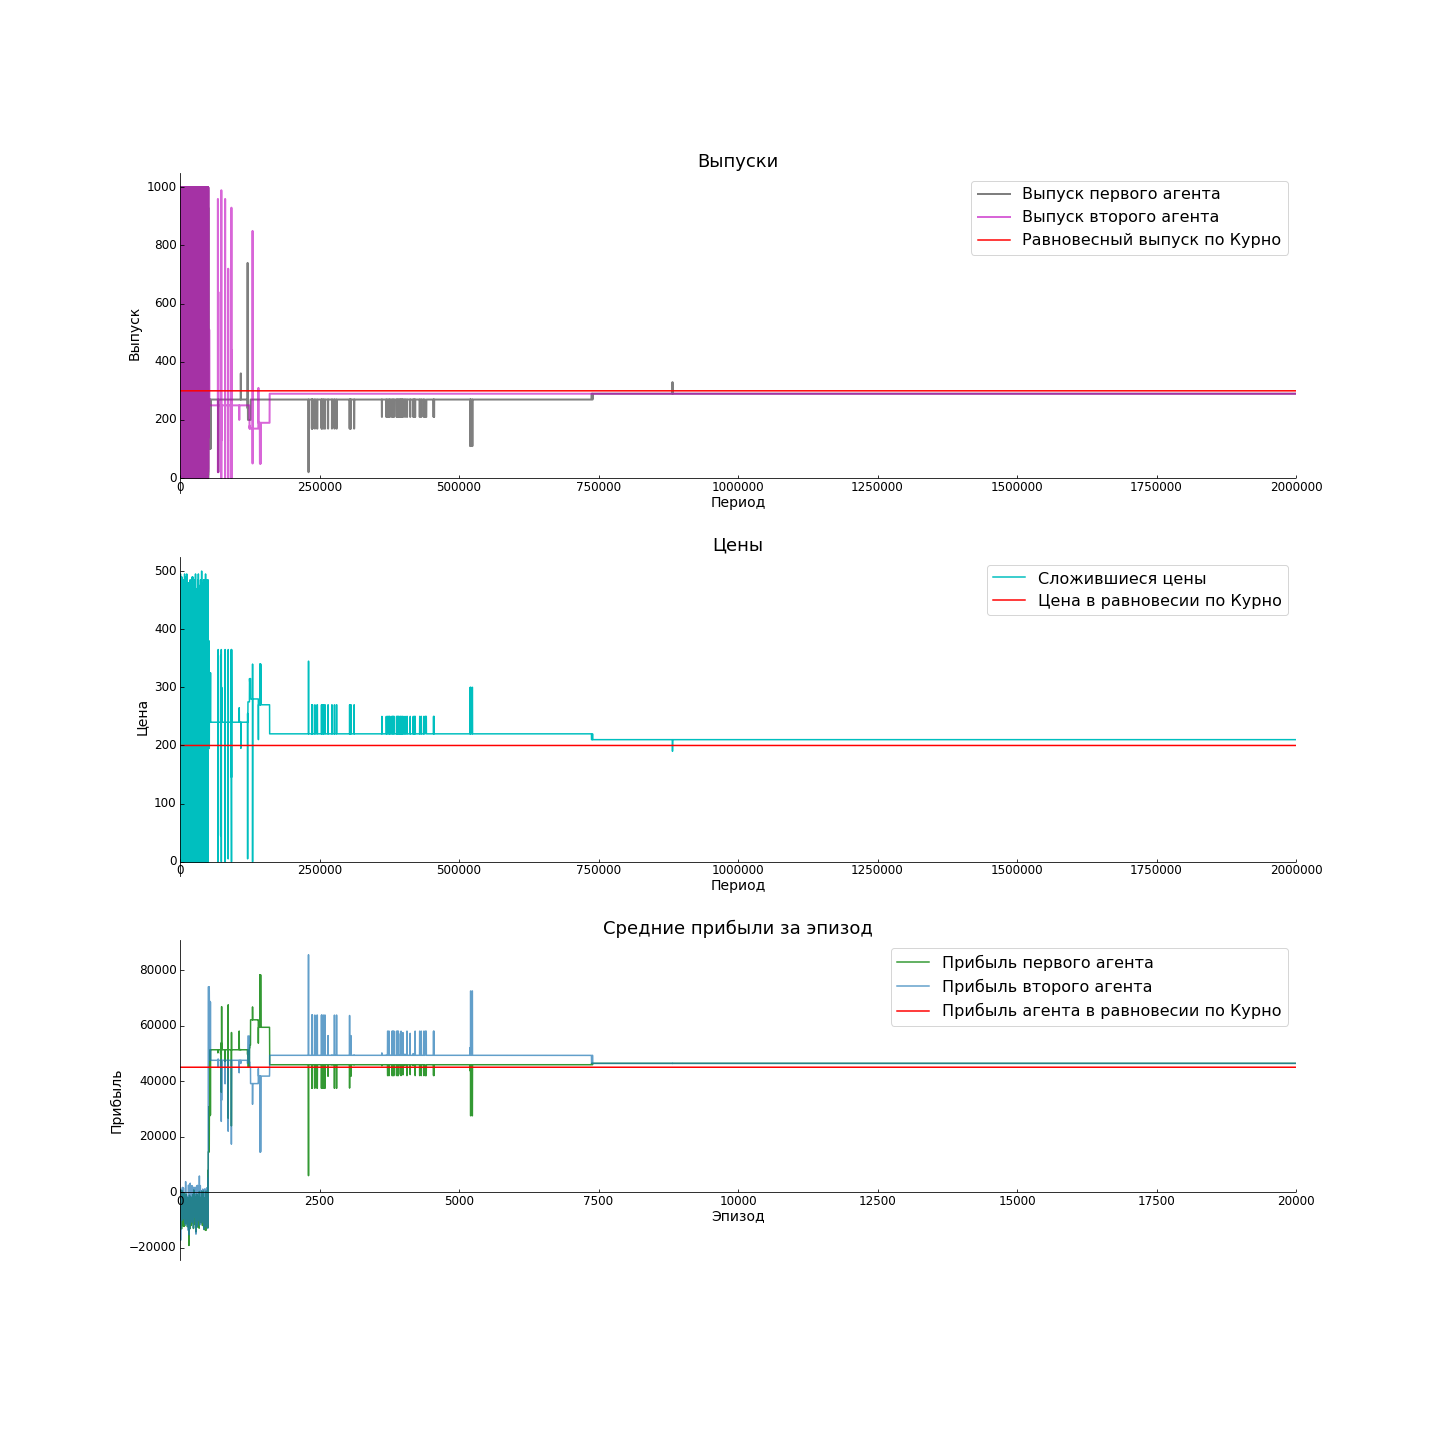
\includegraphics[width=\textwidth,height=\textheight,keepaspectratio]{gamma3.png}
    \caption{$\gamma = 0.3$}
    \label{fig:gamma3}
\end{figure}


На рисунке \ref{fig:gamma3} изображены результаты экспериментов при $\gamma = 0.3$. Хаотичный выбор действий вначале объясняется тем, что агенты начинают обучаться только когда сохраненных траекторий накопится достаточно много. До этого момента их действия выбираются случайно. В отличие от реальных экономических агентов, у них нет априорных знаний о модели, и этот начальный период призван это компенсировать. 

Во всех случаях (больше изображений траекторий обучения можно найти в приложении \ref{priloj}) агенты сходились к определенному равновесию. Кроме того, в этом равновесии по крайней мере один агент всегда получал прибыль больше, чем в случае статического равновесия Курно. Тем не менее, даже в случае нулевого дисконт-фактора статическое равновесие Курно не было достигнуто, что может быть объяснено погрешностью аппроксимации и особенностями обучения. Агенты приобретают слишком большую уверенность в своих действиях до того, как статическое равновесие достигнуто, а поколебать эту уверенность могла бы только новая информация, которую в равновесном состоянии брать неоткуда.
\begin{table}[h]
\centering
\caption{Характеристики статического равновесия Курно}
\label{my-label}
\begin{tabular}{|l|l|l|l|}
\hline
$\gamma$ & Цена & Прибыль 1-го агента & Прибыль 2-го агента\\ \hline \hline
$0$ & $200$ & $45000$ & $45000$ \\ \hline
\end{tabular}
\end{table}
\begin{table}[h]
\centering
\caption{Характеристики равновесия при различных $\gamma$}
\label{my-label}
\begin{tabular}{|l|l|l|l|}
\hline
$\gamma$ & Цена & Прибыль 1-го агента & Прибыль 2-го агента\\ \hline \hline
$0$ & $245$ & $42900$ & $56550$ \\ \hline
$0.3$ & $210$ & $46400$ & $46400$ \\ \hline
$0.6$ & $210$ & $44800$ & $48000$ \\ \hline
$0.9$ & $290$ & $50400$ & $50400$ \\ \hline

\end{tabular}
\end{table}


С точки зрения человека вид траекторий выпуска не отвечает ожиданиям от действий разумных экономических агентов. Это определяется особенностями алгоритма обучения. Во-первых, агенты не учат модель, они учат только действия, которые принесут максимальную полезность в той или иной ситуации. То есть поведение агентов в MADDPG рефлекторное. В то время как реальные экономические агенты могут эксплицитно использовать свое представление о функции спроса и стратегиях других агентов при принятии решения. Во-вторых, агенты в MADDPG учатся исключительно методом проб и ошибок, что связанно с первым пунктом. Они не используют свое знание о модели, чтобы предсказать к каким последствиям может привести то или иное действие, вместо этого они вынуждены его пробовать. Обе эти проблемы можно было бы решить используя обучение с планированием, то есть заставить агентов учить и эксплицитно использовать информацию о модели и стратегиях других агентов при принятии решений. 

\newpage
\section{Заключение}
В данной работе я применил алгоритм MADDPG для обучения агентов в модели динамической олигополии Курно. Обученные агенты сходятся к определенному равновесию. Однако даже при выполнении предпосылок для сходимости к статическому равновесию Курно, оно не достигается. Кроме того, действия агентов во время обучения не похожи на действия рациональных экономических агентов. Для решения последней проблемы в будущих работах по теме, я предлагаю использовать обучение с планированием, когда агенты учат модель и стратегии других агентов, и используют это знание при принятии решений. 

\newpage
\bibliographystyle{unsrt}

\bibliography{ref}
\newgeometry{left=1cm, right=1cm, top=2cm, bottom=2cm, bindingoffset=0cm
}
\section{Приложение} \label{priloj}

\begin{algorithm}
\selectlanguage{russian}

\caption{MADDPG \cite{lowe2017multiagent}}
\begin{algorithmic}[1]
\For{эпизод $= 1$ до $M$}
\State Инициализировать случайный процесс $\mathcal{N}$ для эксплорации
\State Получить начальное состояние $\bold{x}$
\For{$t=1$ до максимальной длины эпизода}
\Stateдля каждого агента $i$ выбрать действие $a_i=\mu_{\theta_i}(o_i) + \mathcal{N}_t$ с учетом текущей стратегии
\State выполнить действия $a = (a_1, \ldots, a_N)$, получить значения вознаграждения $r$ и состояния $\bold{x}'$
\State сохранить $(\bold{x}, a, r, \bold{x}')$ в буфер $\mathcal{D}$
\State $\bold{x}\gets \bold{x}'$
\For{агента $i=1$ до $N$}
\State Получить случайную выборку размера $S$ кортежей вида $(\bold{x}^j,a^j,r^j,\bold{x}'^j)$ из $\mathcal{D}$
\State $y^j \gets r^{j}_i+\gamma Q^{\mu'}_i(\bold{x}'^j,a'_1,\ldots,a'_N)\rvert_{a'_k=\mu'_k(o^k_j)}$
\State Обновить критика, минимизируя фукнцию потерь $L(\theta_i)=\frac{1}{S}\sum_j(y^j-Q^{\mu}_i(\bold{x}^j,a^j_1,\ldots,a^j_N))^2$
\State Обновить актора, используя выборочный градиент стратегии:
\begin{equation}
    \nabla_{\theta_i}J\approx \frac{1}{S}\sum_j\nabla_{\theta_i}\mu_i(o^j_i)\nabla_{a_i}Q^{\mu}_i(\bold{x},a^j_1,\ldots,a_i,\ldots, a^j_N)\rvert_{a_i=\mu_i(o^j_i)} \nonumber
\end{equation}

\EndFor
\State Обновить параметры целевой нейросети для каждого агента i:
\begin{equation}
    \theta'_i \gets p\theta_i + (1-p)\theta'_i \nonumber
\end{equation}
\EndFor
\EndFor
\end{algorithmic}
\end{algorithm}
\begin{figure}[h]
    \centering
    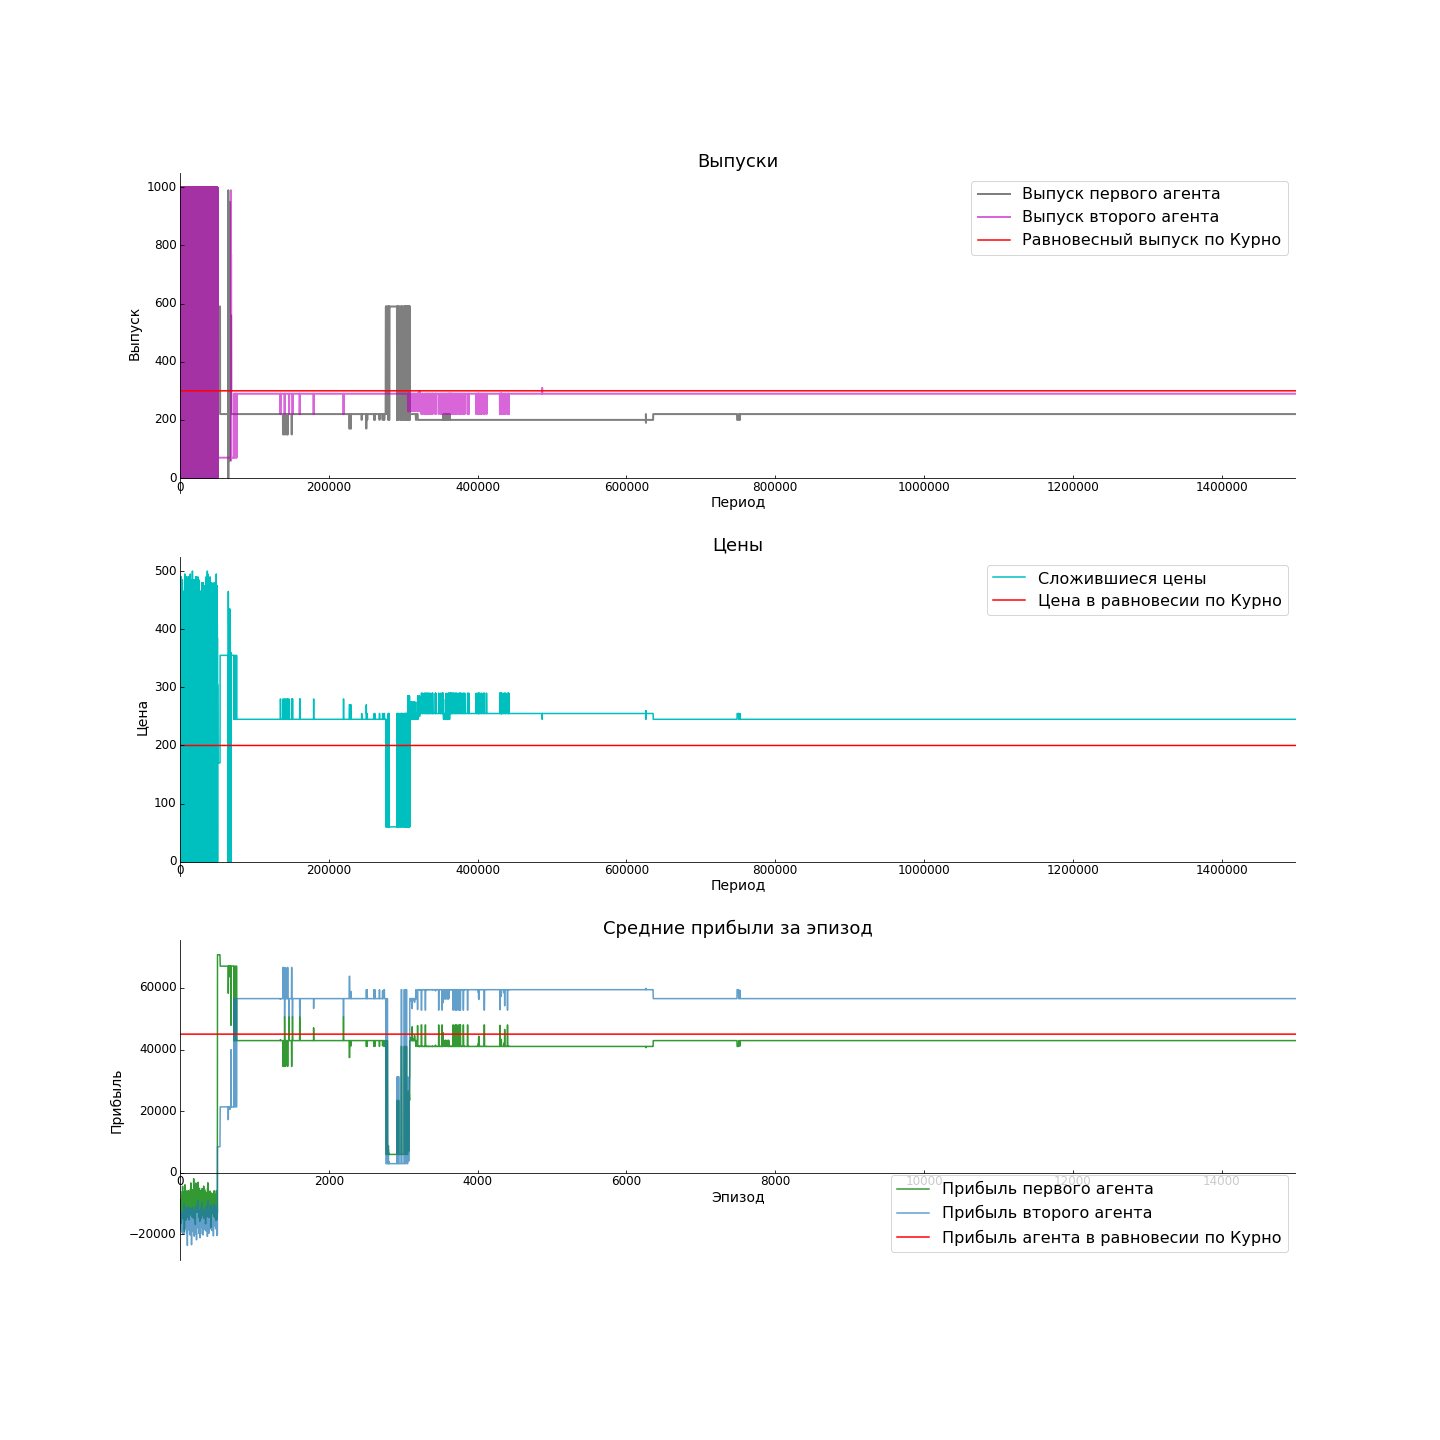
\includegraphics[width=\textwidth,height=\textheight,keepaspectratio]{no_gamma.png}
    \caption{$\gamma = 0$}
    \label{fig:gamma0}
\end{figure}

\begin{figure}[h]
    \centering
    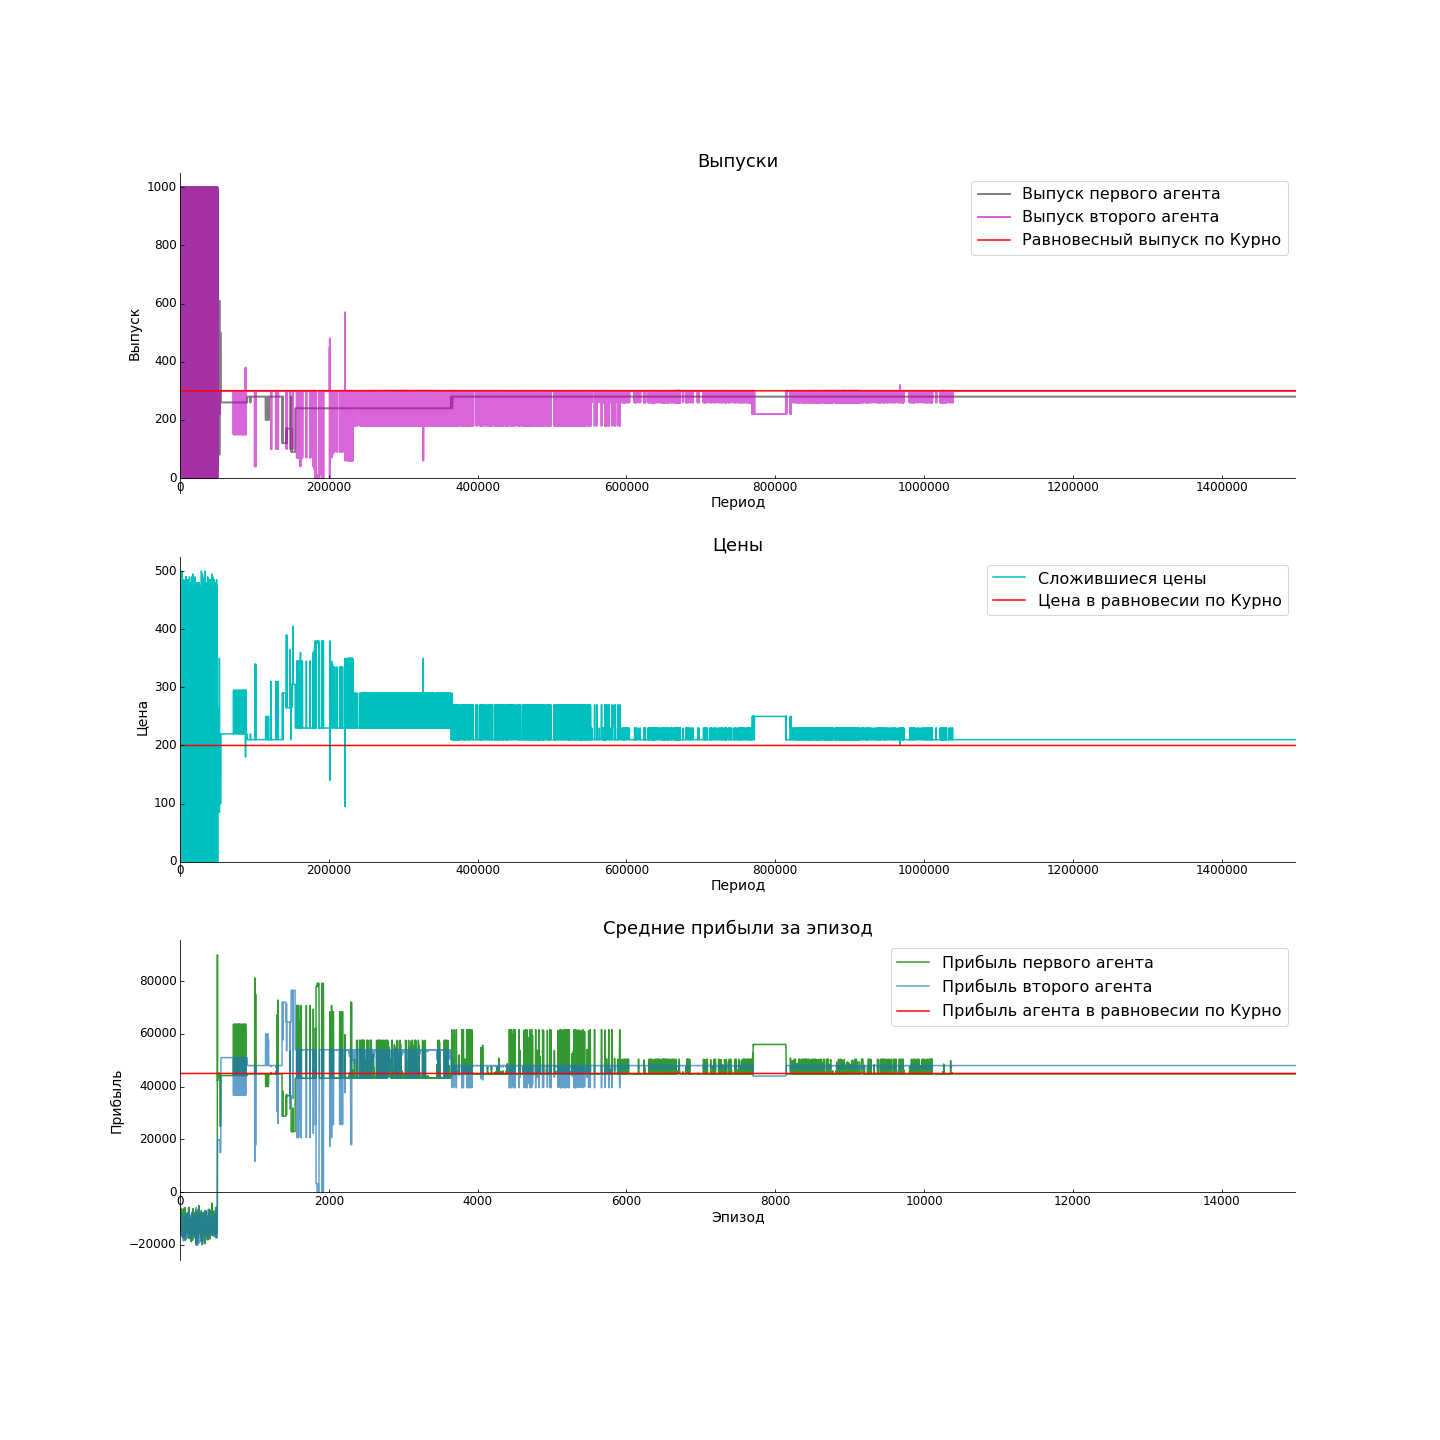
\includegraphics[width=\textwidth,height=\textheight,keepaspectratio]{gamma_6.png}
    \caption{$\gamma = 0.6$}
    \label{fig:gamma6}
\end{figure}


\begin{figure}[h]
    \centering
    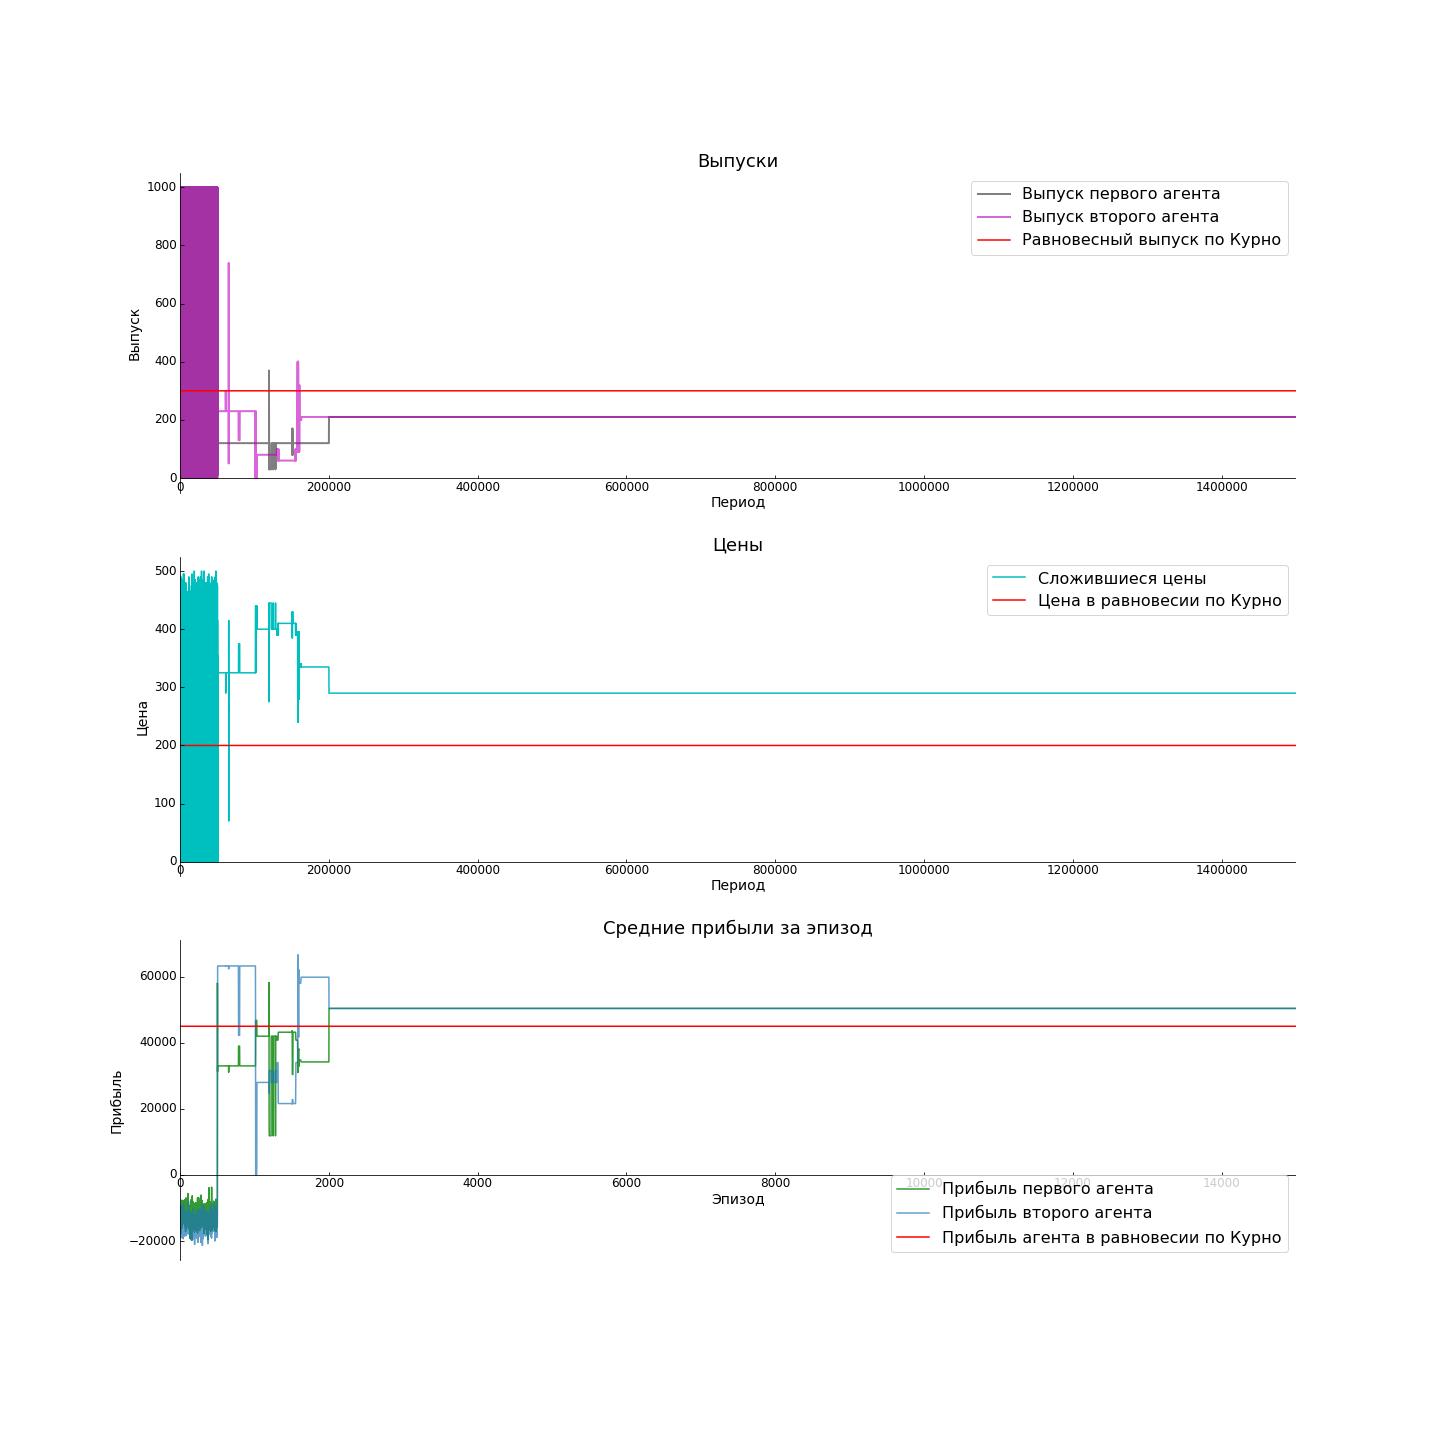
\includegraphics[width=\textwidth,height=\textheight,keepaspectratio]{gamma_9.png}
    \caption{$\gamma = 0.9$}
    \label{fig:gamma9}
\end{figure}
\end{document}
